		\section{Биотический фон в сообществах {\it Macoma balthica}}

	\subsection{Белое море}
Описание сообществ макробентоса проводили на 6 мониторинговых участках в Кандалакшском заливе отдельно на каждом мареографическом уровне. 
Таким образом, всего было получено $12$ таксономических списков.
Всего на  исследованных участках было обнаружено $57$ таксонов беспозвоночных (приложение~\ref{app:species}, таблица~\ref{tab:White_species}).
Из них только непосредственно {\it Macoma balthica} встречена во всех 12 описаниях.
$18$ таксонов из $57$ были представлены только в одном описании.
Количество таксонов в одном описании колебалось от $5$ в верхнем горизонте материковой литорали в Лувеньге до $42$ у нуля глубин в Южной губе о.~Ряшкова.
По количеству таксонов преболадали представлители Polychaeta (22 таксона).

Классификация участков по видовому составу была проведена при помощи кластеризации методом ближайшего соседа по коэффициенту Жаккара. 
Достоверность кластеров оценивали с помощью анализа сходства профилей (SIMPROF) (\cite{Clarke_et_al_2008}).

При анализе фаун с выделением горизонтов было выделено 6 групп участков ($p<0,05$) (рис.~\ref{ris:cluster_white_species_tidal}). 
	\begin{figure}
		\begin{center}
			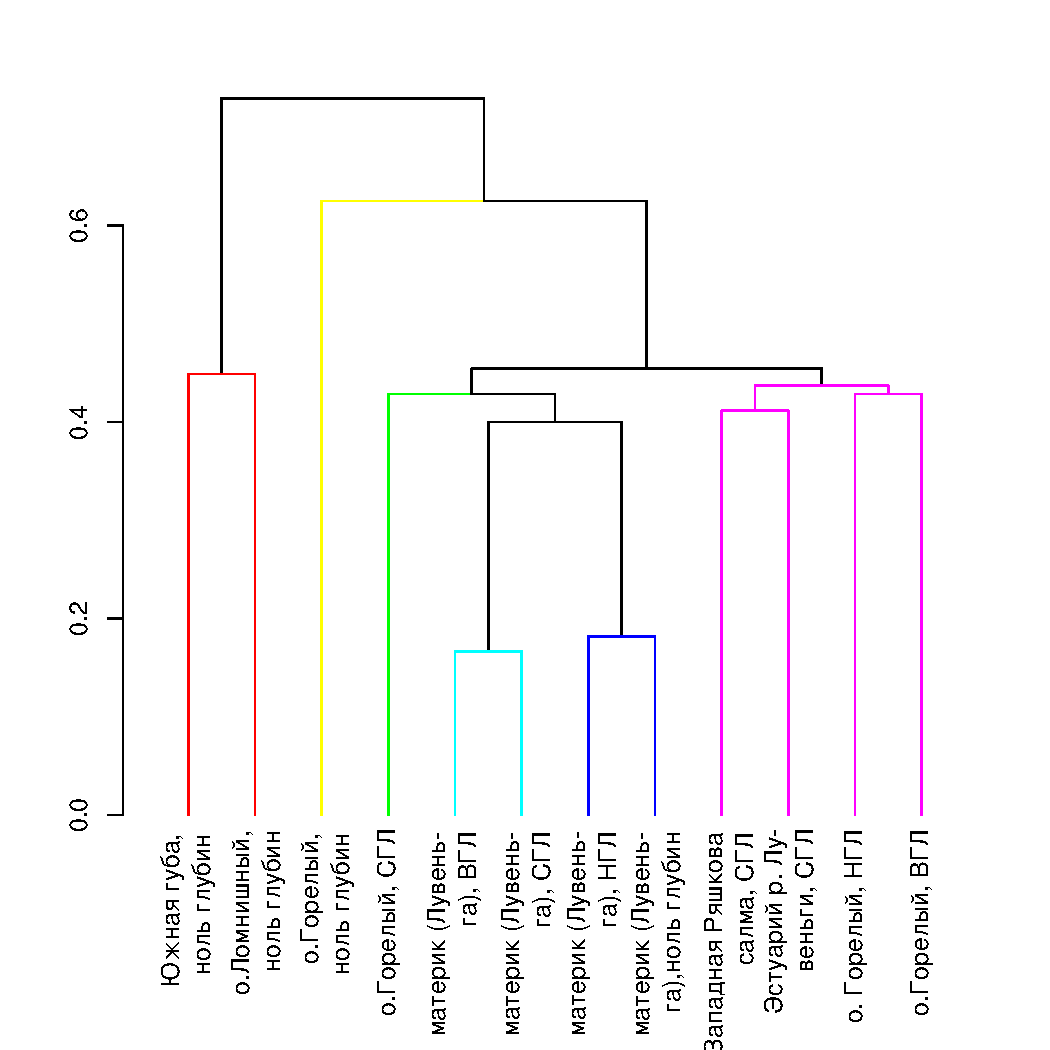
\includegraphics{../White_Sea/soobshestvo/White_fauna_tidal_jaccard_single_1.pdf}
		\end{center}
	\caption{Классификация отдельных горизонтов литорали по видовому составу}
	\label{ris:cluster_white_species_tidal}

	\footnotesize{Кластеризация по методу ближайшего соседа с использованием коэффициента Жаккара. По оси ординат --- коэффициент Жаккара. Цветом показаны кластеры, достоверно выделяющиеся при 5\% уровне значимости.}
	\end{figure}
Группировка станций по кластерам неоднородна. 
Три кластера демонстрируют сходтво по географическому признаку (голубой, синий и, отчасти, фиолетовый на рис.~\ref{ris:cluster_white_species_tidal}), три по мареографическому признаку (красный, синий и голубой кластер на рис.~\ref{ris:cluster_white_species_tidal}), остальные не показывают явной приуроченности.


При анализе фаун отдельных участков было выделено три группы (рис.~\ref{ris:cluster_white_species_sites}.) 
	\begin{figure}
		\begin{center}
			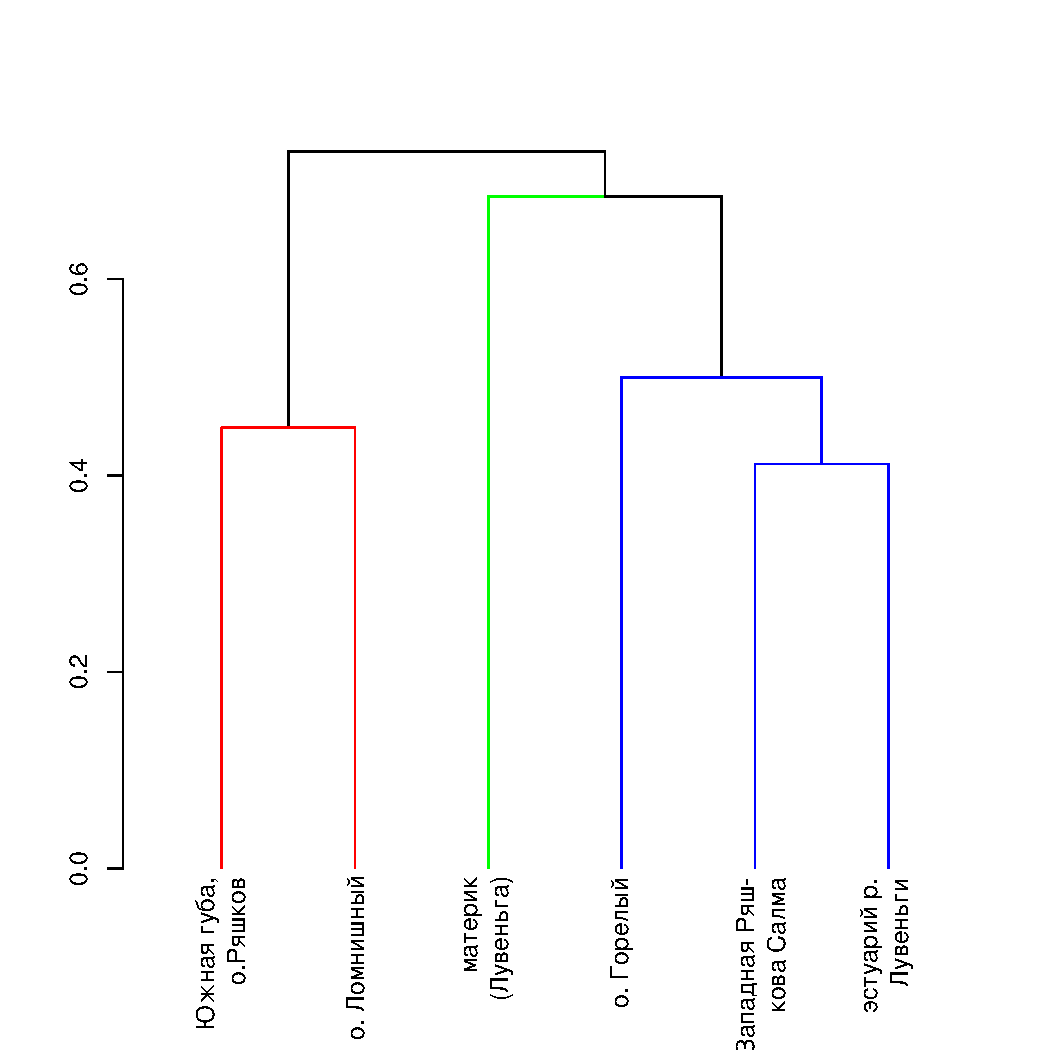
\includegraphics{../White_Sea/soobshestvo/White_fauna_sites_jaccard_single_1.pdf}
		\end{center}
	\caption{Классификация участков по видовому составу}
	\label{ris:cluster_white_species_sites}

	\footnotesize{Кластеризация по методу ближайшего соседа с использованием коэффициента Жаккара. По оси ординат --- коэффициент Жаккара. Цветом показаны кластеры, достоверно выделяющиеся при 5\% уровне значимости.}
	\end{figure}
Первый кластер образуют сообщества в  Южной губе о.~Ряшкова и на о.~Ломнишный, которые близки как географически, так и мареографически (исследованы сообщества у нуля глубин).
В отдельный кластер попадает материковая литораль в районе Лувеньги, что связано, по-видимому, с максимальным биотопическим разнообразием на данном участке, поскольку здесь в пределах ограниченного участка представлены как илисто-песчаные пляжи верхней и нижней литорали, так и заросли фукоидов и взморника.
Участки на о.~Горелый, в эстуарии р.~Лувеньги и на островной литорали Западной Ряшковой салмы формируют третий кластер.
От выделяется характеризуется наименьшим внутренним сходством, однако участки, где исследовали только средний горизонт литорали (Западная Ряшкова салма и эстуарий р.~Лувеньги) более сходны между собой, чем попадающий в тот же кластер о.~Горелый.

	\subsection{Баренцево море}

Всего на исследованных участках нами было обнаружено $48$ таксонов беспозвоночных (приложение~\ref{app:species}, таблица~\ref{tab:Barents_species}). 
При этом в пределах каждого из горизонтов литорали были встречены все таксоны. 
Более трети таксонов ($17$ из $48$) - это редкие виды (встречены в одном описании), и лишь {\it Macoma balthica} встречается во всех описаниях. 
Количество таксонов на участке колебалось от $6$ (верхняя сублитораль губы Ивановская) до $22$ (средний горизонт литорали губы Дальнезеленецкая). 
По соотношению таксонов на всех участках преобладали Polychaeta.
	
Классификация участков по видовому составу была проведена при помощи кластеризации методом ближайшего соседа по коэффициенту Жаккара. 
Достоверность кластеров оценивали с помощью анализа сходства профилей (SIMPROF) (\cite{Clarke_et_al_2008}).

При анализе отдельных горизонтов литорали было выделено два кластера: сублитораль губы Ивановская и литораль всех остальных учатсков (рис.~\ref{ris:cluster_barents_species_tidal}). 
	\begin{figure}
		\begin{center}
			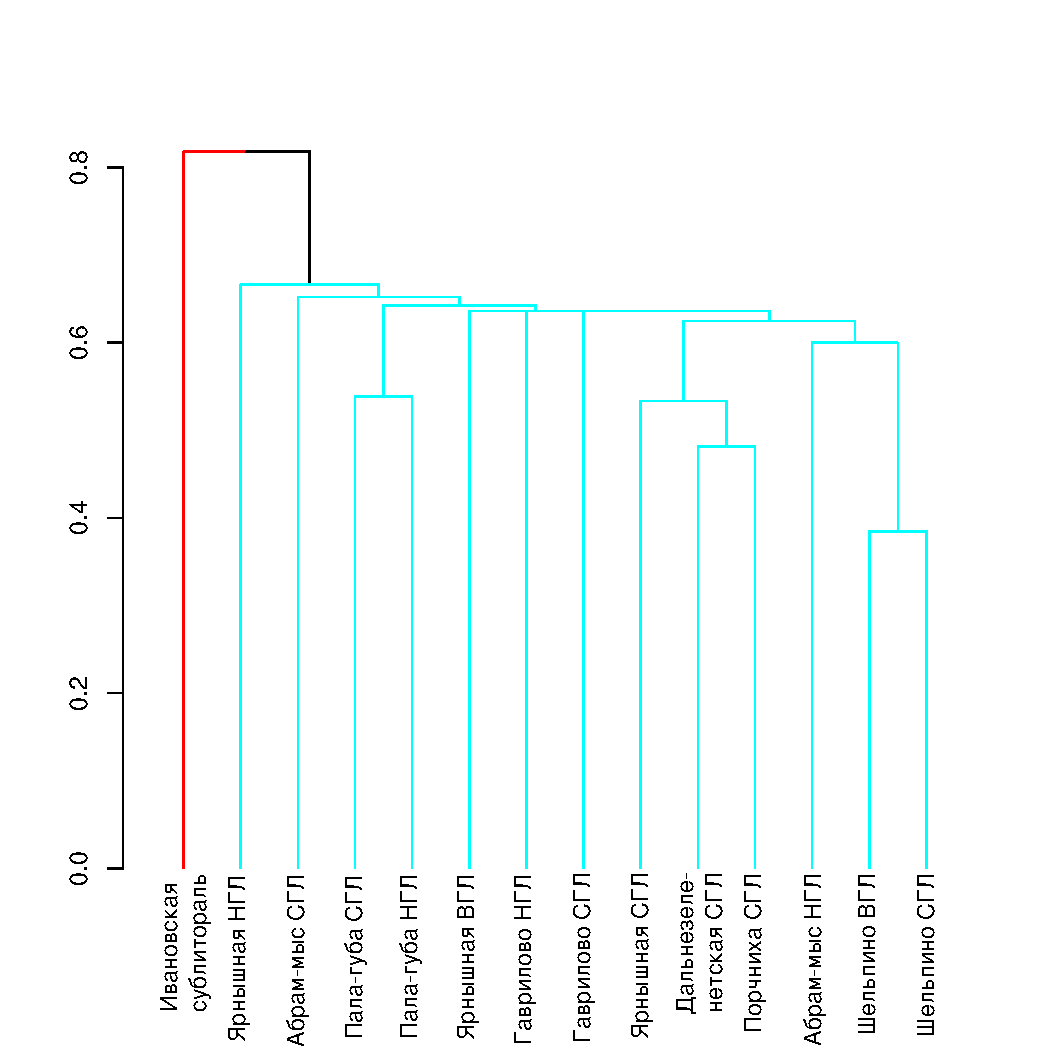
\includegraphics{../Barenc_Sea/soobshestvo/Barents_fauna_tidal_jaccard_single_1.pdf}
		\end{center}
	\caption{Классификация отдельных горизонтов литорали по видовому составу}
	\label{ris:cluster_barents_species_tidal}

	\footnotesize{Кластеризация по методу ближайшего соседа с использованием коэффициента Жаккара. По оси ординат --- коэффициент Жаккара. Цветом показаны кластеры, достоверно выделяющиеся при 5\% уровне значимости.}
	\end{figure}

Возможно, что была выбрана слишком дробная единица анализа, и посмотрим как распределятся полные описания сообществ по изученных участкам литорали (рис.~\ref{ris:cluster_barents_species_sites}. 
	\begin{figure}
		\begin{center}
			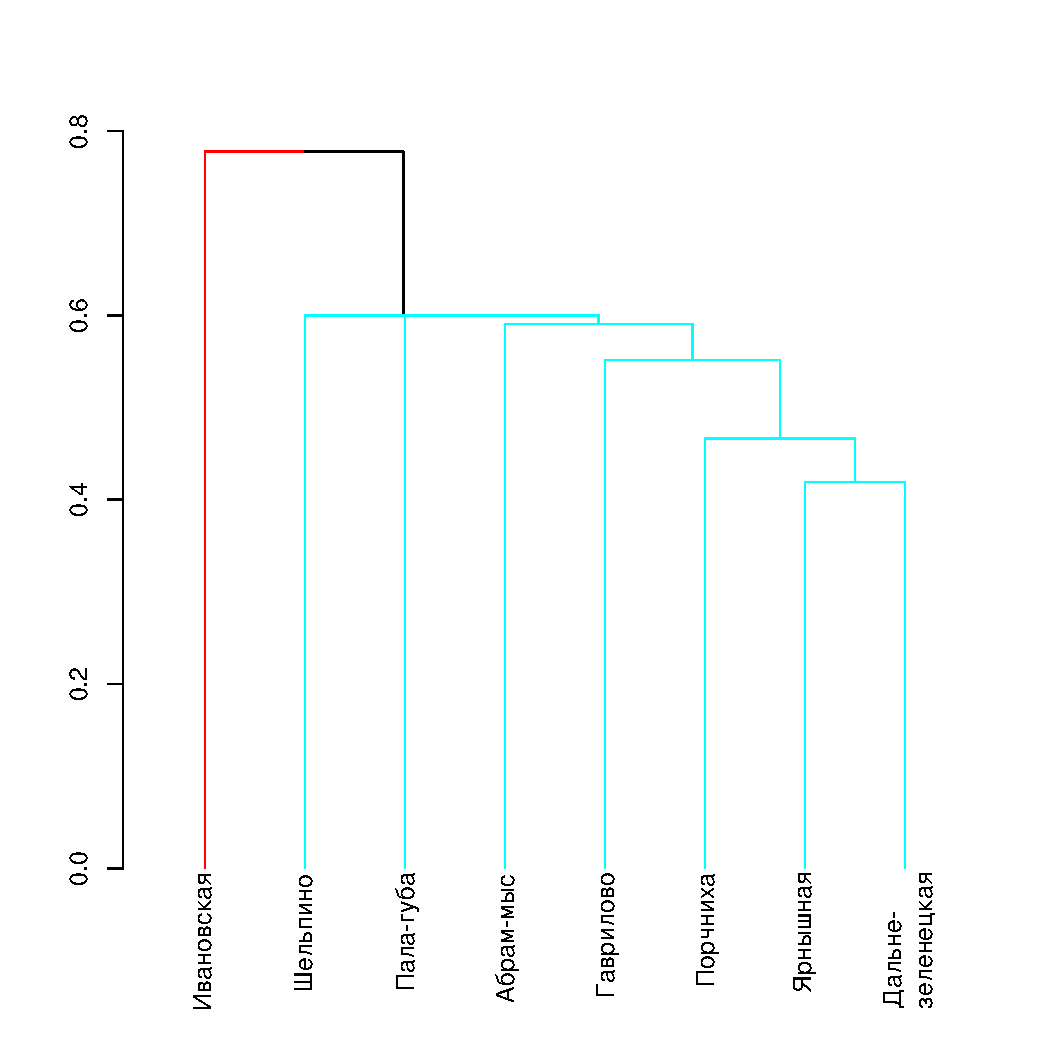
\includegraphics{../Barenc_Sea/soobshestvo/Barents_fauna_sites_jaccard_single_1.pdf}
		\end{center}
	\caption{Классификация участков по видовому составу}
	\label{ris:cluster_barents_species_sites}

	\footnotesize{Кластеризация по методу ближайшего соседа с использованием коэффициента Жаккара. По оси ординат --- коэффициент Жаккара. Цветом показаны кластеры, достоверно выделяющиеся при 5\% уровне значимости.}
	\end{figure}
Результат аналогичен, достоверно отличается только фауна губы Ивановская.

Влияние фактора гранулометрического состава грунта на состав сообщества было оценено с помощью анализа сходства ANOSIM. 
Градации фактора были заданы как илисто-песчаная, песчаная и гравийно-песчаная литораль, а в качестве меры сходства использовали коэффициент Жаккара. 
В результате не было обнаружено достоверного влияния данного показателя на видовой состав сообщества ($R=0,053, p=0,36$).
	
Таким образом, таксономический состав сообществ на исследованных участках достаточно вариабелен, и по-видимому, сходство определяется географической близостью участков. 

%была еще тема на конференции в Мурманске. Не надо ли добавить оттуда и пересчитать все нафиг.
